\documentclass{article}
\usepackage{graphicx}
\usepackage{afterpage}
\usepackage{setspace}

\begin{document}

\begin{titlepage}
    \centering
    \includegraphics[width=12cm]{images/20090516224137!Logotip_KBTU (1).jpg}
    
    \vspace{0cm} % Add vertical space
    {\fontsize{40}{48}\selectfont Факультет Информационных систем} % Large font size and the text you mentioned
    
    \vspace{0.1cm} % Add vertical space
    
    \begin{center} % Center the following text
        Faculty of Information Technology\\
        Department of Electrical Engineering and Computer Science
    \end{center}
    
    \vfill % Fill the vertical space
    
    {\LARGE\bfseries Laboratory Work \#3}\\
    {\LARGE\bfseries Comprehensive Circuit Analysis and Measurements}
    
    \vspace{4cm} % Add vertical space
    
    \begin{flushright}
        Done by: Sagingaly Meldeshuly \\
        Checked by: Raushan Amanzholova \\
        September 2023
    \end{flushright}
    
    \vfill % Center the page number vertically
    \begin{center}
        2023, Almaty
    \end{center}
    
\end{titlepage}



% "*" убирает нумерацию в разделе section
% "$ $" в долларах мы пишем математических операций
% " \times " это умножение с крестиком
% P_R_2=$I_R_2 \times V_R_2$
% \[ numerator and denominator
%\frac{a}{b}
%\]
% power ^
% \subsection подтопик
% Omega
% \\ is used to create a new line or break a line. It's similar to pressing "Enter" or "Return" on your keyboard when you're writing a regular text document.
\begin{flushleft}
\textbf{Purpose of the work laboratory work:}
\end{flushleft}
\begin{enumerate}
    \item Start you second project in Ni MultiSim.
    \item Measure the corresponding voltages,currents and powers for each part of the circuit.
    \item To apply advanced circuit analysis techniques, including Thevenin, Norton, and superposition theorems, and to validate theoretical results with practical measurements using the Elvis Evaluation Board.
\end{enumerate}

\begin{flushleft}
\textbf{Brief theory}
\end{flushleft}

\begin{flushleft}
In electronic circuit analysis, various techniques can simplify and solve complex circuits:

Thevenin's theorem allows us to replace a network of resistors and sources with a single voltage source and a series resistor.

Norton's theorem enables the representation of a network with a single current source in parallel with a resistor.

Superposition theorem states that the response (voltage or current) in any branch of a linear circuit with several independent sources equals the algebraic sum of the responses caused by each source acting alone, while all other sources are turned off.

Additionally, Kirchhoff's laws (KCL and KVL) provide fundamental constraints for current and voltage in circuits. Practical implementations may reveal deviations due to component tolerances, measurement accuracies, and other real-world factors.
\end{flushleft}

\begin{flushleft}
\textbf{Pre lab tasks}
\end{flushleft}

\begin{flushleft}
First source: $R = (2 * 10^8)/(3*10^4) + 5 * 10^4 = 17/3 * 10^-^4  \Omega$\\
    $i_1 = i = (7 * 3) /(17 * 10^4) = 1.235 A$\\
    $i_3 = i_1 * 4/5 = 0.988 * 10^-^4 A$\\
    $i_2 = i_1 - i_3 = 0.247 * 10^-^4 A$\\

    Second source: $i_4 = 15/ (15 * 10^3) = 1 mA$\\ 
    $R = (5 * 10^3 * 2 * 10^4) / (2.5 * 10^4) + 10^4 = 14 * 10^3 \Omega$\\
    $i_3 = 10 / (14 * 10^3) = 1.0714 * 10^-^3 A$\\
    $i_1 = 2/3 * i_3 = 0.714 * 10^-^3 A$\\
    $i_2 = i_3 - i_1 = 0.357 * 10^-^3 A$\\

    Total: $i_4 = 15/ (15 * 10^3) = 1 mA$\\
    $i_1 = 5.905*10^-^4 A$\\
    $i_2 = 3.818 * 10 ^-^4 A$
    $i_3 = 9* 10^-^4 A$
    \break \break
\end{flushleft}



\begin{flushleft}
1) Find the currents on resistors by using Superposition    
\end{flushleft}
\begin{flushleft}
    \begin{titlepage}
    \centering
    \includegraphics[width=10cm]{images/photo1695462997.jpeg}
\end{flushleft}

\begin{flushleft}
2) Find the voltage on R1 by using Thevenin. Find the voltage on R4 by using Norton.
\begin{flushleft}
    \centering
    \includegraphics[width=10cm]{images/photo1695464380.jpeg}
\end{flushleft}

\begin{flushleft}
\textbf{In lab tasks}
\end{flushleft}




Connect your circuit to Elvis Evaluation Board, and get measurements. Compare with in- lab results.

\begin{flushleft}
    \begin{titlepage}
    \centering
    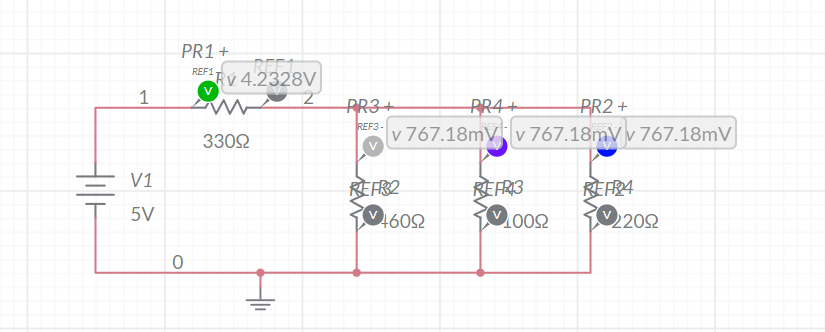
\includegraphics[width=14cm]{images/image (5).png}
\end{flushleft}



\begin{flushleft}
    \begin{titlepage}
    \centering
    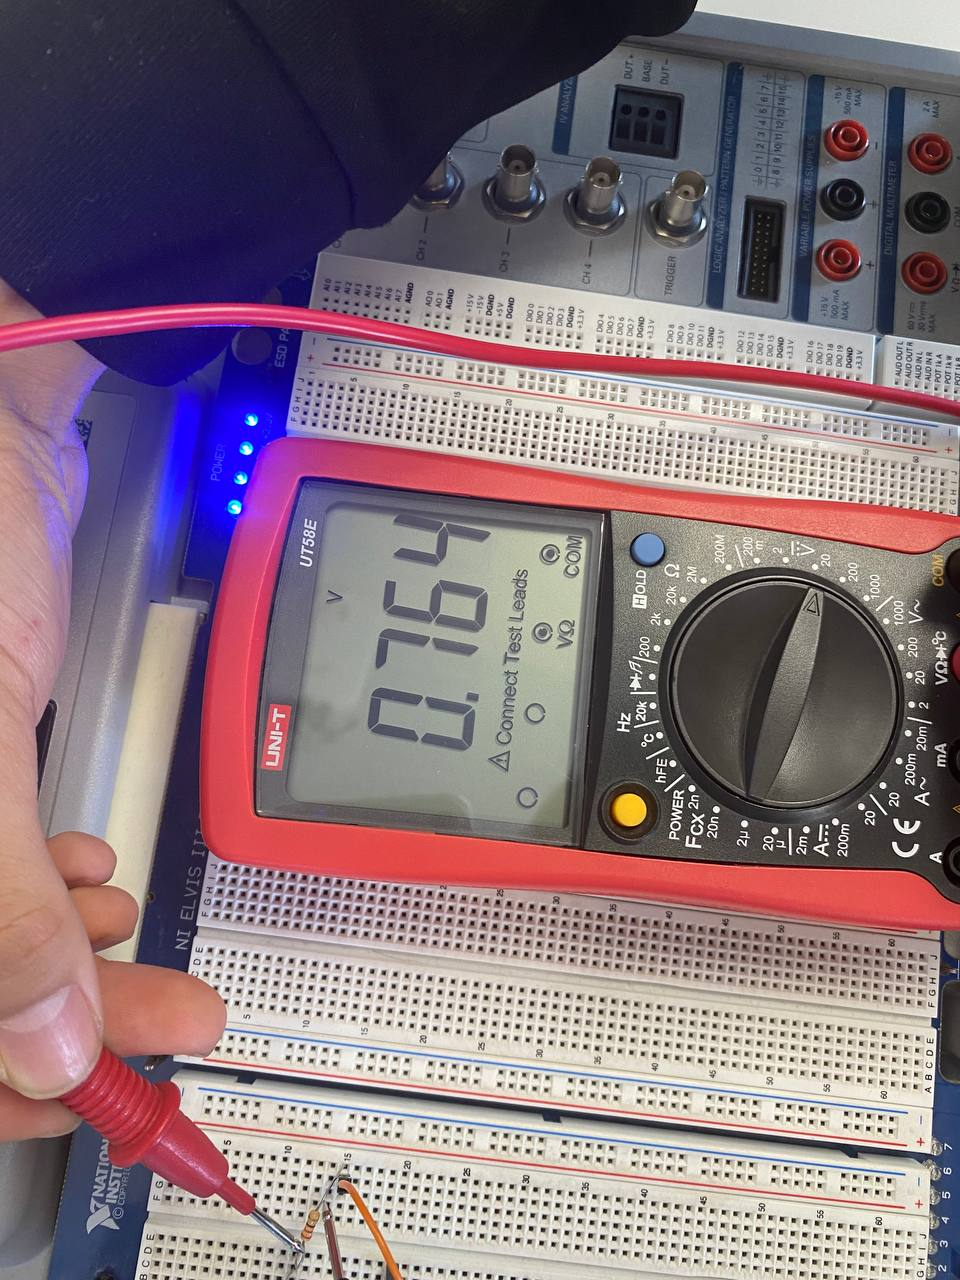
\includegraphics[width=10cm]{images/photo1696237774 (5).jpeg}
\end{flushleft}

\begin{flushleft}
    \begin{titlepage}
    \centering
    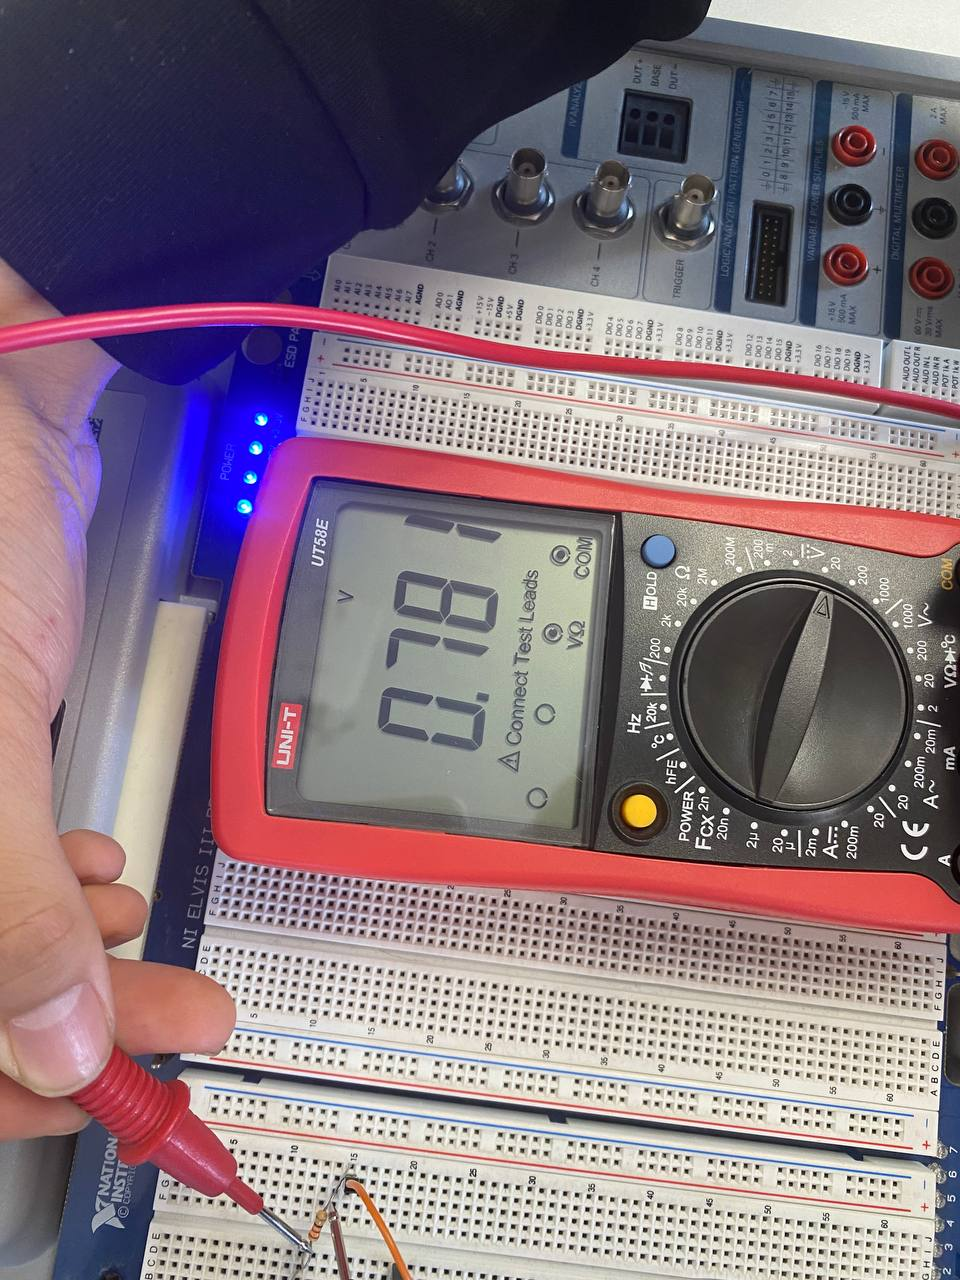
\includegraphics[width=10cm]{images/photo1696237774 (6).jpeg}
\end{flushleft}

\begin{flushleft}
    \begin{titlepage}
    \centering
    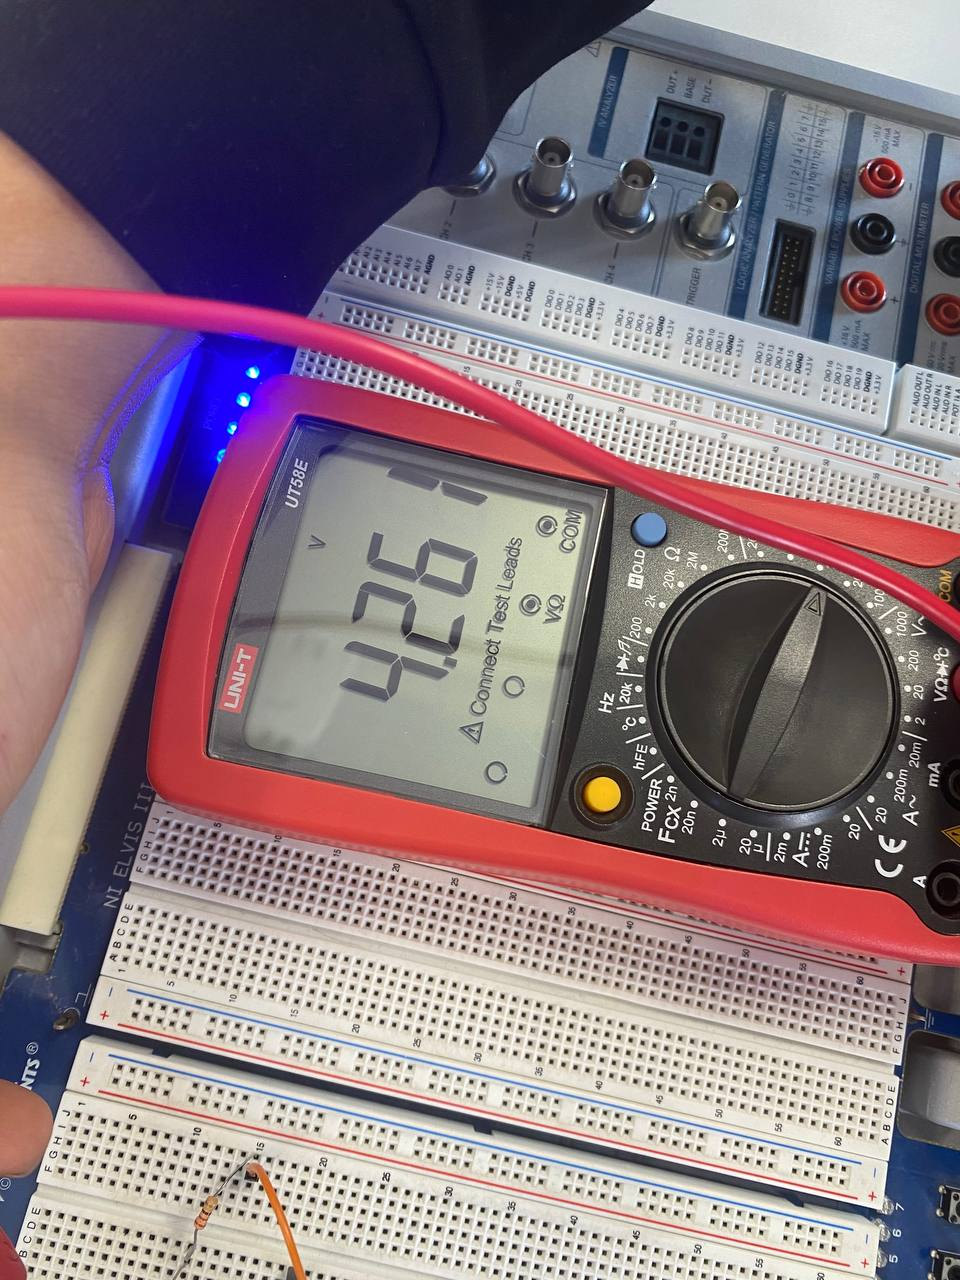
\includegraphics[width=10cm]{images/photo1696237774 (7).jpeg}
\end{flushleft}

\begin{flushleft}
    \begin{titlepage}
    \centering
    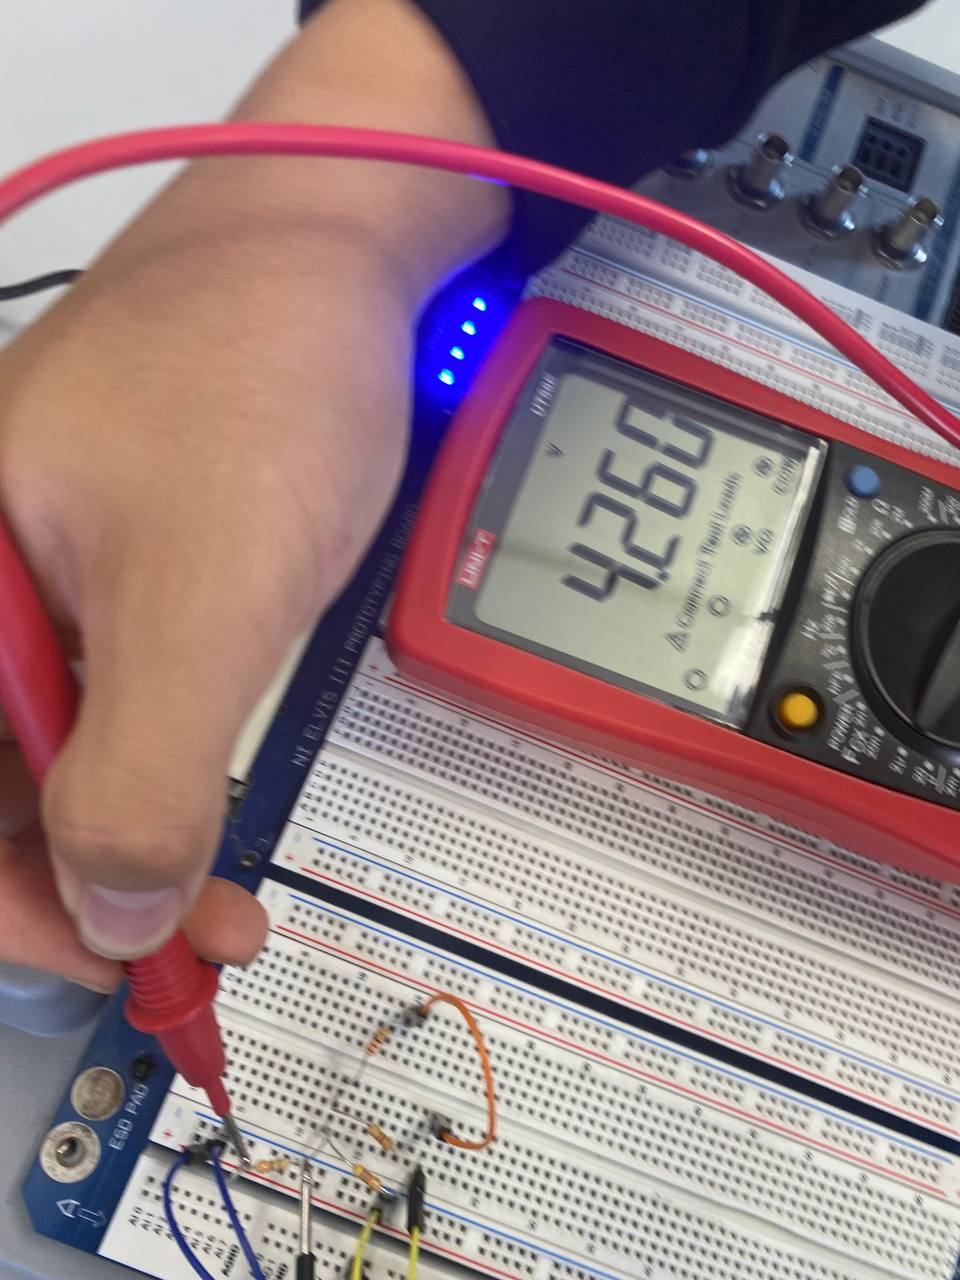
\includegraphics[width=10cm]{images/photo1696237774 (8).jpeg}
\end{flushleft}


\begin{flushleft}
    \begin{titlepage}
    \centering
    \includegraphics[width=10cm]{images/image.png}
\end{flushleft}

\begin{flushleft}
\begin{table}[h]
    \centering
    \begin{tabular}{|c|c|c|c|c|c|c|c|c|c|c|}
        \hline
        V_R_1 & V_R_2 & V_R_3 & V_R_4 & I_R_1 & I_R_2  & I_R_3  & I_R_4  & I_V_1  \\
        \hline
    6.5714V  & -13.571v & -8.4286v & 15.000v & 328.57 & -1.6857mA & -1.3571mA  & 1.000mA &  2.6857mA \\
        \hline
    \end{tabular}
    \label{tab:sample_table}
\end{table}
\end{flushleft}

\begin{flushleft}
    \centering
    \includegraphics[width=10cm]{images/lab.png}
\end{flushleft}

\begin{flushleft}
\begin{table}[h]
    \centering
    \begin{tabular}{|c|c|c|c|c|c|c|c|}
        \hline
         V_R_1 & V_R_2 &V_R_3 & V_R_4 & V_R_5 & MY\\
        \hline
        0.89V  & 6.81V & 5.92V & 5.89V & 0.187V & TABLE\\ 
        \hline
         I_R_1 & I_R_2 & I_R_3 & I_R_4 & I_R_5 & I_V_2\\
        \hline
        0.89mA & 0.681mA & 1.185mA & 294,5mA & 1,8660mA & 1.57mA\\
        \hline
    \end{tabular}
    \label{tab:sample_table}
\end{table} 
\end{flushleft}

\begin{flushleft}
\noindent \textbf{Post lab}
\end{flushleft}
1. Find currents that goes through R3, R1 and V2 by using Thevenin. Find the currents that goes through R2 and R4 by using Norton.
\begin{flushleft}
    \begin{flushleft}
    \centering
    \includegraphics[width=10cm]{images/laboratory.png}
\end{flushleft}
\end{flushleft}
\begin{flushleft}
\textbf{Conclusion:}
\end{flushleft}

 
\begin{flushleft}
In this laboratory work, we embarked on a project within Ni MultiSim, which provided an excellent platform for circuit design and analysis. Our primary objectives encompassed the measurement of voltages, currents, and powers associated with different components of the circuit. To achieve this, we applied advanced circuit analysis techniques, including Thevenin's theorem, Norton's theorem, and the superposition theorem.

 

The provided theoretical background introduced us to invaluable tools in electronic circuit analysis. The Thevenin theorem, which simplifies complex networks of resistors and sources into a single voltage source and a series resistor, offers an efficient means to streamline circuit analysis. Norton's 


Additionally, we acknowledge the fundamental role of Kirchhoff's laws (KCL and KVL) in imposing constraints on current and voltage within circuits. These laws form the backbone of circuit analysis, providing essential principles for analysis and design. It is essential to recognize that practical implementations may introduce deviations due to component tolerances, measurement accuracies, and real-world factors. These deviations highlight the importance of practical experimentation and measurements, which were central to our laboratory work.


\end{flushleft}
\end{document}
